\subsection{SEMICONDUCTING QUANTUM DOTS}

Due to their practical application and rather easy, yet not really repeatable fabrication, semiconductor quantum dots have made a vast impact in all technology. Their potential confinement in all three directions allows to profit from many new possibilities, not known in solid state physics before.
We can easily distinguish three different categories for their production which are:
\begin{itemize}
\item Self assembled QDs
\item Colloidal QDs
\item Electrostatically definded QDs 
\end{itemize}
Considering the fact that we are only using the second ones, we will mainly focus on them. 

\subsubsection{COLLOIDAL QUANTUM DOTS}
To put it straightforward, CQDs are semiconductor crystal of nanometre scale size, with diameter less than twice the Bohr radius, which are synthesized(deployed) by nucleation in colloidal solutions. They are surrounded and restricted by surfactant molecules called ligands. 

\begin{figure}[H]
\centering
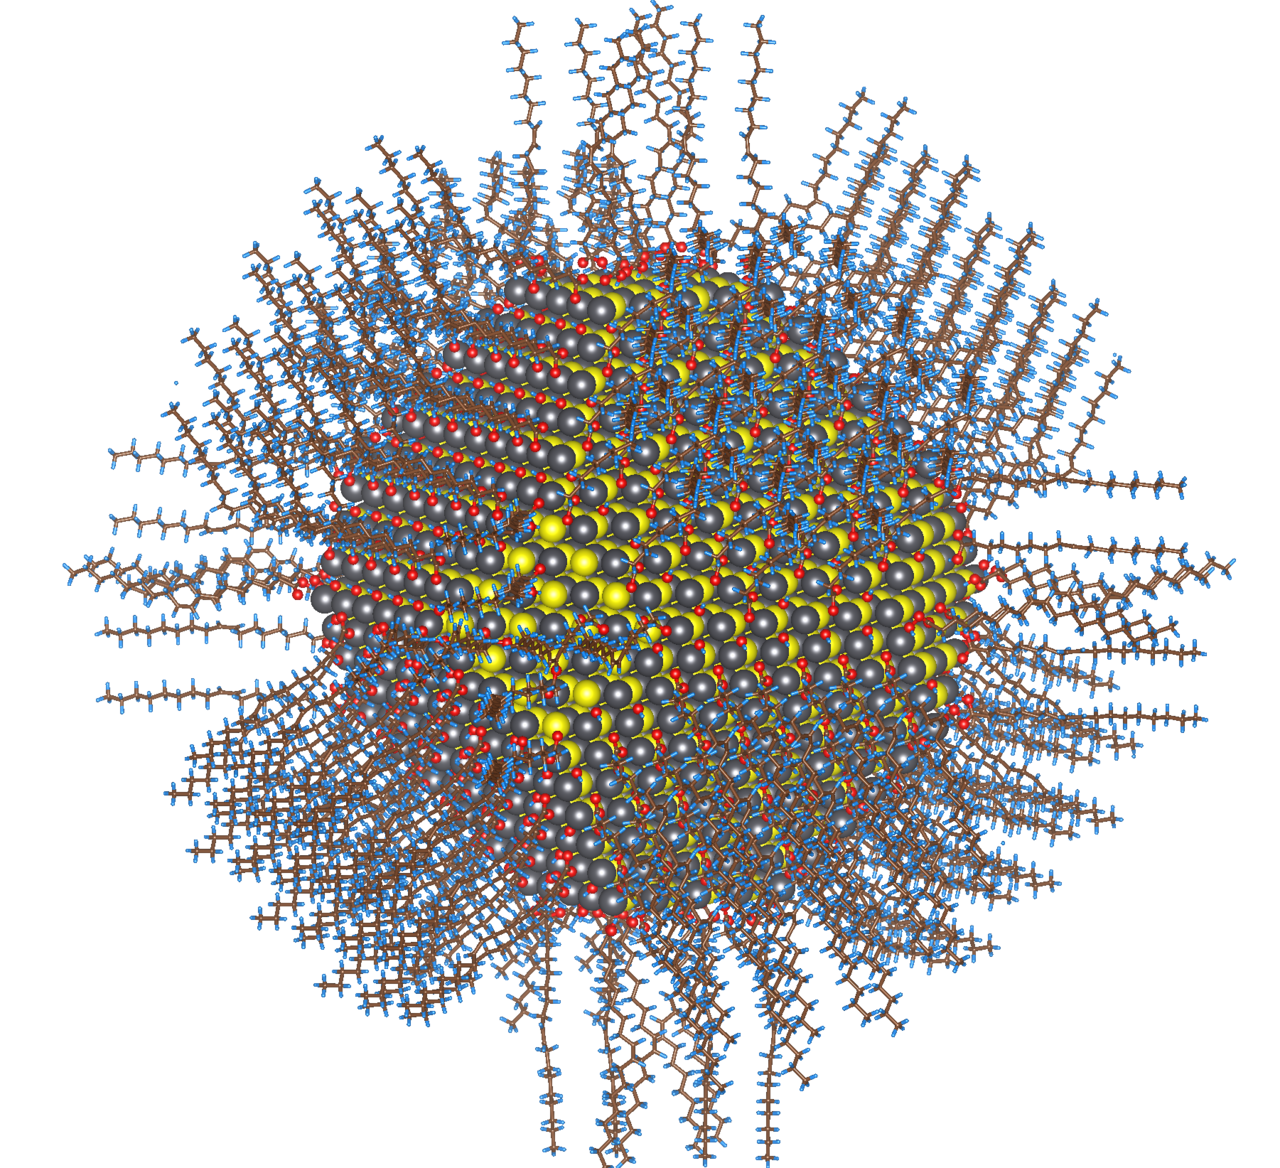
\includegraphics[width=0.4\textwidth]{ch2/colQD}

\caption{Image of ideal CQD composed of selenide with passivation with oleic acid, oleyl amine and hydroxyl ligands \cite{qd}}
\end{figure}

\noindent They have manifested to provide a development of numerous types of optoelectronic devices including photo-diodes and PV devices. The properties of CQDs are easily adjusted by changing the volumetric features of nanoparticles similarly to metallic nanoparticles in plasmonic transport. \cite{Abdelhady2015} \cite{G.D.Scholes2003}

\noindent Even though we don't focus on the synthesis of particular used CQDs, it is instructional and scientifically appropriate to be slightly familiar with it. It consists of three-component solutions, which are precursors, organic surfactants and solvents. In order for get the precursors transformed into single chains called monomers, the probe is heated to high temperature(they have enough energy to get separated), then, when there's enough of them, the monomers are growing into crystals. Of course, the temperature shall be manipulated with a dose of care because when it's too high the crystals aren't forming fine or at all. When we achieve optimal saturation of monomers, we get quite even growth of all particles, (small ones grow faster than the heavy ones) and it has to be sustained in order for the homogeneity to be achieved.
Typically, CQDs create alloys, binary or ternary, and contain 100 to $10^5$ atoms. Usually, they confine all carriers inside the volume.
\subsubsection{Quantum dot size}
With changing the size of the nanoparticle we can control the band gap over significant range of spectrum. Yet, practically, the width of the nanoparticle is estimated from the energy band gap.
 \cite{Yu2003}
 
\subsubsection{Quantum dot shape}
The geometry in physics plays an important role, there is no question about that. It is obviously not different for Quantum Dots. The quantum confinement strongly depends on the shape and dimensional geometry. The ability to control the growth of certain form allows the nanoparticles to exhibit a variety of properties. 

\subsection{CORE-SHELL CQDS}     
Modification of the standard synthesis methods allows us to create new behaviour and improvements in nano-structures characteristics. For example, in this method, same type, but different semiconducting nano-crystals are grown around the first ones(core). They tend to achieve better luminescence than the former because we simply drastically cut the possibility of non-radiative recombinations between energy levels. We can differ type 1 structures using conduction band of the core below the shell energy level(the core confines all carriers inside because of the energy minimisation) and in the second type, the energy levels are mixed so only one type of carriers is confined to the shell and the core. \cite{phdsemi}

\begin{figure}[ht]
\centering
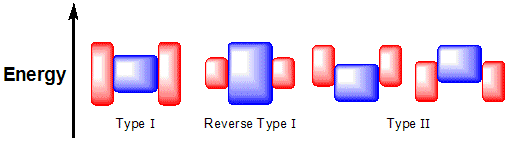
\includegraphics[width=0.8\textwidth]{ch2/Core_shell_types}
\caption{Types of Core-Shell CQDs(blue color is core energy structure), we can see that in the first type both electrons(smallest energy in CB) and holes(biggest energy in VB) are confined beneath the core. \cite{coreshell}}
\end{figure}

\subsection{CQD SUPER-CRYSTAL}
With CQDs we can even create super-lattices(layers of few materials which create a periodic structure). In order to achieve the fine quality of them we need to have an absolutely outstanding transport properties. \cite{tranSupLat}
\subsubsection{Further reading for CQDs}
More about synthesis and theory of nano-crystals and thermodynamics can be read in \cite{Klimov}, \cite{crystal}

\subsection{PRINCIPLES OF QDSCS}
Quite early, because in fair 1960s, the idea of harvesting sunlight with using sensitized semiconductor devices with generation of carriers inside narrow band semiconductors has been proposed. The usage of colloidal quantum dots has produced new possibilities and and shown amusing prospects for using nanotechnology. The properties can be tuned by changing the QDs size itself which means changing the size of electronic band (relocate CB - conduction band and VB - valence band) depending mainly on effective masses of the carriers. The electronic shift that we can achieve by relatively simple parameters manipulation will provide a shift of VB edge downwards and CB upwards, as a result of a, quite important in this scale, quantization of energies. As we know, besides band gap enlarging, it also changes the driving force for carries injection and this is most important part, as we want to use them as an amplifier in the PV devices. The great achievement of these types of solar cells is the decoupling the charge generation and its transport to different materials- the hole and electron transport layers. The effect of such a procedure is the decrease in recombination process and reduction of production costs.  Without that technique, the architecture is adequate to the standard PV solar cell device. The generation of electron-hole pairs proceeds the injection of electrons from CB of light harvesting material to electron acceptor layer and holes from VB to hole acceptor layer. We call this process a charge separation. Nevertheless, even though we do regenerate QDs in the light harvesting area after charge separation, we still have to struggle with recombination processes and consider them as the significant performance wasters. \cite{S.Gimenez2009}


There are few commonly used configurations of solar cells based on those previously mentioned nano-crystals and are shown in \ref{fig:confstru}

\begin{figure}[ht]
\centering
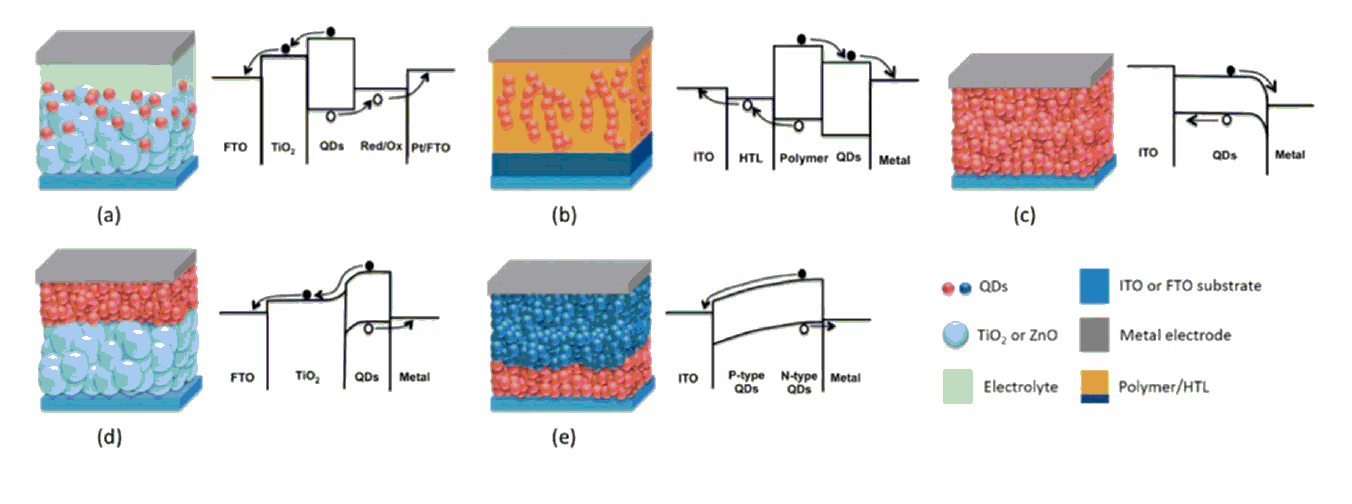
\includegraphics[width=\textwidth]{ch2/confstru}
\caption{Schematic illustration of configurations and band structures of QD solar cells: a) QD-sensitized b) hybrid QD-polymer c) Schottky junction d) p-n hetero-junction e) p-n homo-junction \cite{HuashangRao2018}}
\label{fig:confstru}
\end{figure}

Schottky schematic is a type of device where thin QDs film is placed between two contacts and is used for generating electrons and holes. The barrier, which is created between the low-work metal and QDs layer, is quite similar to bulk one where the potential is bent proportionally because of the charge transfer between the layers that touch. From them, few very unique and promising short currents have been achieved. Unfortunately, low open circuit voltages are present for them because of the pinning of Fermi level. Then, we have the depleted heterojunction, where we use wide band gap oxides such as ZnO on a conducting glass. After that we put some QDs films above that and end it with a fine metal contact. The oxide layer behaves as layer for electron conducting phase, so the metal contact extracts majority carriers. There we have more of a compromise between $I_{sc}$ and $V_{oc}$.  The next type is a hybrid QD-polymer solar cell, where electron is transported and photon absorbed both in the QDs layer(with the polymer film together). The PCEs of such attitudes to the device engineering is still smaller than the former ones, probably due to not optimal hole transporting layers. P-n hetero- or homo- junctions are both traditional methods of harvesting and transporting the light but instead of using bulk semiconductors, we use semiconducting QDs. 

The Quantum Dots Sensitized Solar Cells(QDSCs) are devices in which QDs are not the most important part when considering the carrier transport. The idea was to replace dyes with QDs, but the rest of components has been still based on the concepts formed by their ancestor. Sadly, not to late after, it was realised that it's not so similar at all and some of the components need to be redesigned from scratch. However, even though the DSCs are easier to achieve the better performance with, the QDSCs are more promising and theoretically can be cheaper and have longer lifetime. Inside the device structure, the QDs itself are responsible for light absorbing and carriers creation. Then they are divided in different layers so obviously the great PCE can only be achieved if large incident photon to current efficiencies(IPCE), $V_{oc}$ and fill factor are possible. 

\begin{equation}
IPCE(\lambda ) = LHE(\lambda ) \phi_{inj} \eta_{col}
\end{equation}

Where $\eta_{col}$ is electron collection efficiency, $\phi_{inj}$ is electron injection efficiency and of course $LHE(\lambda )$ is left to be the light harvesting efficiency, so it's directly connected to absorption and automatically to QD loading and the band gap, as has been seen in theory chapter. The loading only depends on the quantitative parameters of transport oxide layers such as thickness, particle size and coverage degree. The injection then depends on how fine would we attach both layers together and the collection efficiency will consider the interfaces and the internal structure of transporting phases. Of course this means, as in all of the solar cells, high mobility with relatively slow recombinations in the main energy regime. We can now clearly see that the big advantage of those cells is that they separate the ideas of charge generation and transport to different parts, so it gives more possibilities to engineer new materials. 
\cite{HuashangRao2018} \cite{Wu2014}

\subsection{MATERIALS AND PERFORMANCE DEVELOPMENT OF QDSSC - A REVIEW}

\begin{enumerate}

\item \textbf{Electron Transporting Materials(ETM)}

They are used to support charge separation as briefly described above.The function proceeds as a support for QD in the charge generation layer, as it transports charged electrons to the conductive substrate(usually ITO or FTO). \cite{X.Gao2017} \cite{Tian2015} The properties shall be as follows:
\begin{itemize}
\item
  Matching CB edge which will determine exciton generation and
  partial transfer efficiency.
\item
  High electron mobility.
\item
  Fine surface to provide suitable loading of particles.
\item
  Suitable technological properties, such as stability, low cost etc.
\end{itemize}

The most widely studied materials nowadays are TiO2 and ZnO. Materials based on the first one are of such importance due to their non-toxicity, chemical stability and low cost \cite{I.Mora-Sero2014a} \cite{Tian2015} . Among them (TiO2-NP) based mesoporous layers are researched as photo-anodes \cite{I.Mora-Sero2014a}. The highest efficiency ever recorded(up to 2018) were based on that material \cite{Du2016} \cite{J.Du2017} . Unfortunately, the probability for charge recombination in that kind of films is rather unsatisfactory.  Therefore, one provides one-dimensional structures such as nano-rods and nano-wires to maintain fairly smoother electron transport channel and decrease loses provided with recombination \cite{Y.Liu2014} \cite{M.A.Manthrammel2015} . In 2007 it was shown that TiO2 nano-tubes win over nano-particles of the same material in case of transport capacity \cite{Kamat2009} \cite{Tvrdy2008}.  Thus, the research of such structures was accelerated and many brand new CdSe sensitisation methods were proposed \cite{A.Yamada2010} . After that, many different sensitisations were provided, in which also PbS QDs had their small part \cite{C.Shi2017} . Although promising, the 1D structured TiO2 based anodes were unsatisfactory in case of PCEs, when comparing to standard nanoparticles (maximum of around 6\%  ). The hypothesis was put on insufficient loading amount on 1D structured TiO2, therefore the focus should be put on improvement of that area. A group of researchers has also used graphene frameworks incorporated into TiO2 photo-anode achieving 4.2\% PCE for QDSSCs. \cite{XinMeng2014} By using double-layered films with particles of bigger volume, there has been achieved a high PCE of 4.92\%. A lot of dopants and different solutions, hybrid photo-anode films with metal and non-metal ions and carbonaceous layers has been proposed to improve performance of PV devices. Also with the usage of hollow structure techniques, by creating nano-tube arrays, the possibility of achieving a PCE of 6 \% has been shown \cite{MikhailArtemyev2019}. Improvement in light absorbance was achieved by using microporous TiO2 photo-anode for PbS quantum dot sensitised solar cells achieving up to 3.5\% PCE performance.

In case of ZnO based photo-anodes the differencing property is a higher electron mobility and better conduction band edge. With them, the achievement of higher $V_{oc}$  is more probable \cite{X.Gao2017} . Unfortunately, the chemical stability of those films is significantly lower. Similarly to the former, the nanoparticles were widely studied. \cite{L.Lv2014a} As an example, the CdS sensitised ZnO nanoparticles were used to construct a photo-anode, which allowed the achievement of 4,46\% PCE. They used TiO2 passivation of ZnO surface to improve the PCE of same sensitized CdS/ZnO QDSCs by more than 2\%, achieving 4.68\% \cite{Zhang2013b}. Similarly, the 1D structures for ZnO can be crystallised. The distinction from the former is the ease of it's development. The ZnO nano-wires sensitised with CdSe constructed in 2007 were the launch of the technology development and allowed Young et al. achieve PCE of 4.15\% \cite{J.Qiu2013}. Many more one dimensional structures of ZnO based photo-anodes were used to research maximal performance but it was shown that the problem again concerns the surface area \cite{Gonzalez-Pedro2015}. The second strategy to improve the performance of such material based structures is double layer replacement with two different 1D structures such as NR on bottom and TP on top.  However, the PCEs of ZnO based films still stay behind TiO2 ones.\cite{Zhang2013b}  The Al/Cl hybrid doping allowed to use ZnO in IR spectrum.

There are other kinds of ETMs researched as well.  Using big tandem structures has manifested superb PCE through simulations \cite{GregoryF.Pach2017}. The doping of synergistic fullerene electron transport layer has proven to increase solar cell performance \cite{OleksandrVoznyy2014} . A series of materials such as SnO2, NiO, BiVO4, Zn2SnO4,BaTiO3, CoO have been incorporated to QDSC manifesting future potential. High performance has been achieved using CdS thin films as single-source precursors to ETM layer providing over 8\% PCE. \cite{RobertJ.Patterson2017}

All of the above materials are n-type semiconductors. Furthermore shall we proceed to introduce the p-type metal oxides and p-type Quantum dot sensitised cells. Typically, the NiO semiconductor is widely used. The promising and comprehensive material that can be implemented is CuSCN, which is an inorganic of p-type. Of course, the extraction of a hole from light harvesting layer to a redox couple will be rather slower than in case of electron. Therefore, being the potential solution to this problem, the p-type semiconductor based layers are beginning to leave their mark in PV devices. As expected, the most accurate application of that type of films would be the tandem configuration construction, which contains both n-type and p-type QDSCs to overcome so called  a Shockley-Queisser limit. However appealing, the efficiencies of p-type QDSSCs are yet to be enhanced.

\item \textbf{Hole transporting material (HTM) layers}

The electrolyte or HTM is crucial to QDSSCs as well. The properties of
such film shall be:

\begin{itemize}
\item
  Low corrosivity.
\item
  Red-ox potential appropriate to regenerate QDs and maintain fine
  V\textsubscript{oc} .
\item
  High conductivity through ions.
\item
  Stability and transparency in visible spectrum.
\item
  Possibility to fully regenerate. \cite{HuashangRao2018}
\end{itemize}

The common electrolytes:

\begin{itemize}
\item
  \textbf{Liquid electrolytes}
\item
  \textbf{Quasi-solid state electrolytes}
\item
  \textbf{All-solid state electrolytes}
\end{itemize}

were described comprehensively in the following research papers \cite{HuashangRao2018} \cite{Zhang2015} \cite{Song2017}

Although using Sb\textsubscript{2}Se\textsubscript{3} as a thin light
harvesting film, a group of researchers has also used PbS colloidal
quantum dots as a hole transport layer achieving 6.5\% PCE in 2017 \cite{Wang2017}. Earlier, the usage of graphdiyne(a novel large $\pi$ -conjugated carbon hole transporting material) has allowed an efficient hole transport layer for solar cells based on PbS-EDT colloidal quantum dots\cite{MingjianYuan2016}. Before that, in 2015, colloidal CuInS\textsubscript{2} QDs were layered to hole transporting solution and, even though the scientist did their research on Perovskite solar cell, they accomplished to get almost 8.5\% PCE\cite{JunZhu2015}. The extended device stability and a rise to 10.6\% of PCE was certified using CQD solar cells using P3HT as a hole transport material \cite{Zhang2016}.

\newpage
\item \textbf{QD sensitizers }

The main part of our PV device, the QDSC are QDs. The ability of harvesting interfering light is a crucial component of such device. \cite{Ikeda2014} Therefore, the ideal nano structures should exhibit certain properties:

\begin{itemize}
\item
  A higher conduction band edge than the one in the electron transport material and lower than in hole transport material to provide effective charge separation.
\item
  Obviously, as in all semiconductor PV devices, we shall provide a
  material with accurate band gap, ideal for our purpose. The reason is
  clear, we are interested in superb absorption in wide range of solar
  spectrum.
\item
  The stability is the crucial property as well.
\item
  From the technological point of view - the simple preparation and of
  course low toxicity would be rather expected.
\end{itemize}
Therefore, we will now examine methods to deposit them and the
differences between certain QDs materials.

\textbf{Deploying on the surface}

Because of QDs being inorganic and possessing larger size than simple
molecular dyes, they are much more difficult to tether onto metal oxide
to form a high quality mono layer. Therefore high QD-loading amount is
rather high to achieve. We can difference the deposition methods by
putting them into two categories: \emph{in situ} and \emph{ex situ} . In
the first one, the QDs are grown directly on the surface of the metal
oxide substrate, being created using an ionic precursor. We can include
chemical bath deposition(CBD) and successive ionic layer adsorption and
reaction(SILAR) into this category. The second approach bases on pre
synthesising of QDs and then depositing them onto the metal oxide.
Easily processable and finely reproducible, the in situ method has been
used more widely than its' counter. In that kind of deposition we can control not only the QD-loading amount but also size distribution.
Unfortunately, the achieved density of trap states is rather high, therefore the obtained maximal PCE is about 7\% \cite{L.Lv2014} . In this case, excluding the QDs growth process, we have to accurately deploy them onto the surface. The most common methods are: direct absorption, linker-molecule-assisted self-assembly, electrophoretic deposition. \cite{HuashangRao2018}

\textbf{Ligands}

The ligand part in QDs is, as mentioned before, the important part of obtaining high efficiency of QDSCs \cite{Shang2016}. The comparison of halide ligands in PbS CQDs for field effect transistors(FETs) has been made by researchers in 2018\cite{Balazs2018}. The capping-ligand-induced self-assembly method was the clue for TiO\textsubscript{2} photo-anodes\cite{HuashangRao2018}. Nevertheless, researchers haven't discovered a satisfying approach yet. In 2012, the deposition method were optimised through using ligand-exchange techniques.\cite{Cheng2012} Thanks to that, the PCE record of 13\% was achieved \cite{W.Feng2018} . Not only CLIS deposition has been used. The aqueous solution provided the simplification of QDs fabrication with shorter ligands. Some relatively high PCEs have been achieved with that method. Then, the organic  molecules usage allowed scientist in 2015 to achieve 3 times bigger PCE compared to common creation of PbS quantum dots.\cite{Infante2015} The certified PCE of 11.21\% has been achieved via so called ``solvent curving'', which is the simplified method of PbS QDs fabrication processing. The passivation of PbS QD surface with
L-glutathione was used to produce QDSSCs with promising results.\cite{Cordes2016} 10.6\% PCE was achieved thanks to solvent-polarity-engineered halide passivation \cite{OleksandrVoznyy2016} .


\textbf{Binary structures}

Up to date, binary QDs have also been used as sensitizers. There are
many examples but the most common are: InP, InAs, CdS, CdSe, CdTe,
Ag\textsubscript{2}S and with them, the most interesting one considered
in our case - PbS.\cite{P.Zhao2015} \cite{Y.Yu2008} The main problem with
them is to control and balance the narrower band gap and relatively high
conduction band edge. For example, for PbS nano crystals the band gap is
narrow, but the conduction band edge is rather low, which causes the
problem and has to be dealt with. In case of binary QDs we have to
balance between the light harvesting efficiency and efficiency of charge
injection. Mixing binary structures (for example PbS with PbSe) has been
also proven to enhance the interesting efficiency\cite{ShujuanHuangb22019} \cite{Fan}. Treatment of PbS QDs with metal salts provided some advantages in CQD PV devices resulting in the increase of short circuit current and fill-factor \cite{Maurano2016} .
The crucial part of success in getting high efficiency would also be
suitable engineering of solvent\cite{YuehuaYang2017}.

\textbf{Core shell QDs usage}

The other methods to use QDs as sensitizers in PV devices is creating a
Core/Shell QDs. Their unique properties have been mentioned before. The
alignment in these provides ability to tune the light-absorption range,
recombination processes and charge separation. Usage of them in QDSCs is
rather modern. The first noticed implementation was created by Lee et
al. in 2009. Through SILAR method, he achieved PCE of 4.22\% \cite{Lee2009}. Yet the difficulties in creating specific materials may occur, because of inability to prepare a stable precursor for deposition methods. 

\textbf{Alloyed QDs usage}

The massive perspective in PV devices has also been established by using Alloyed QDs. These allow us to create the non-linear band gap \cite{Regulacio2010} . Stability in such materials is again much higher than in their constituents. A lot of scientific research was done in that area.

\textbf{Doping}

We can also include dopants to QDs. There were a handful of propositions in the \cite{HuashangRao2018} review. Yet, the promising idea has been introduced with the usage of metallic nanoparticles dopants by considering plasmonic physical phenomena.\cite{Kubo2015} \cite{YongjieWang2017}

\newpage
\item \textbf{ Counter electrode}

As we may already expected, they are also playing an important role in
achieving high performance of PV device. The electrodes have to catalyse
reduction reaction. These shall poses properties as follows:

\begin{itemize}
\item
  Good conductivity
\item
  High catalytic activity
\item
  Fine stability, either chemical and physical
\end{itemize}

We can also put them into four categories:

\begin{itemize}
\item
  \textbf{Noble metals}
\item
  \textbf{Metal chalcogenides}
\item
  \textbf{Carbon materials}
\item
  \textbf{Composite CEs}
\end{itemize}
\end{enumerate}
Recent progress has been comprehensively described in those publications.
\cite{Yang2017} \cite{HuashangRao2018} .